\documentclass[11pt]{article}
\usepackage[a4paper, total={6in, 8in}]{geometry}
\usepackage[export]{adjustbox}
\usepackage[utf8]{inputenc}
\usepackage{hyperref}
\usepackage{graphics}
\usepackage{amssymb}
\usepackage[english]{babel}
\usepackage{amsmath}
\usepackage[classfont=bold]{complexity}
\usepackage{tikz}
\usepackage{amsthm}
\usepackage[ruled, linesnumbered, noend]{algorithm2e}
\renewcommand{\thealgocf}{}
\usetikzlibrary{arrows,automata}


\hypersetup{
    colorlinks=false
}
\urlstyle{same}
\graphicspath{ {./images/} }
\everymath{\displaystyle}

\title
{%
  {\Huge CS412 Final Project \\
  \Huge Travelling Salesman Problem\\
    \huge Implementations and Analysis of Various Solutions}
}
\date{\Large \today}
\begin{document}
\maketitle
\centering
\includegraphics[scale=0.2]{images/title.png}
\newpage
\paragraph{}
\paragraph{}
\paragraph{}
\paragraph{}
\paragraph{}
\paragraph{}
\paragraph{}
\paragraph{}
\paragraph{}
\par \centering
This page is has been intentionally left blank intentionally \paragraph{}
The typo in the sentence above is left unfixed intentionally as well, because leaving a page intentionally blank makes the same amount of sense as leaving a typo in a sentence intentionally unfixed. 
\par \flushleft

\newpage
\tableofcontents

\newpage


\newpage
\section{Introduction}
The travelling salesman problem has a long history of being a problem of interest in the field of algorithms. It has garnered much attention and there has been a lot of work that has been done on it. In this project we will set out to establish the details of this problem and why it is so tough. We will then investigate 4 algorithms that have become well known in being useful for solving this problem. One of them produces an exact solution and the rest use approximation techniques. We will be using theory and implementation to test the runtimes of this problem and will then present our research in an appropriate format.
\subsection{Proof: TSP $\in$ NP-hard}
\section{Design Techniques}
	\subsection{Exact Solution}
	The exact solution of the travelling salesman problem requires that that each Hamiltonian cycle is travelled and the minimum path of those cycles is found. However, this is an extremely large problem as there will be $n!$ cycles for a complete graph of size $n$. The dynamic programming approach called the Held-Karp algorithm reduces this time complexity to $O(n^22^n)$. It does so by dividing the problem into sub problems.  A very simple method is to visulize this idea using a tree. \paragraph{}
	Let us begin this explanation, without loss of generality, with a complete graph, $K_4,$ that does not contain loops. 
\begin{center}
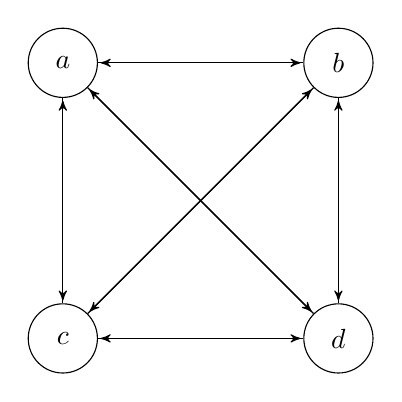
\begin{tikzpicture}[->,>=stealth',shorten >=1pt,auto,node distance=3.5cm,scale = 1,transform shape]

  \node[state] (a) [] {$a$};
  \node[state] (b) [right of=a] {$b$};
  \node[state] (c) [below of=a] {$c$};
  \node[state] (d) [below of=b] {$d$};

  \path (a) edge              node {} (b)
        (b) edge              node {} (a)
        (a) edge              node {} (c)
        (c) edge              node {} (a)
        (a) edge              node {} (d)
        (d) edge              node {} (a)
        (b) edge              node {} (c)
        (c) edge              node {} (b)
        (b) edge              node {} (d)
        (d) edge              node {} (b)
        (c) edge              node {} (d)
        (d) edge              node {} (c);

\end{tikzpicture}
\end{center}
Starting from vertex a, or any vertex to maintain generality, we can build a decision tree that traverses each path, this represents the the power set of the graph
\begin{center}
    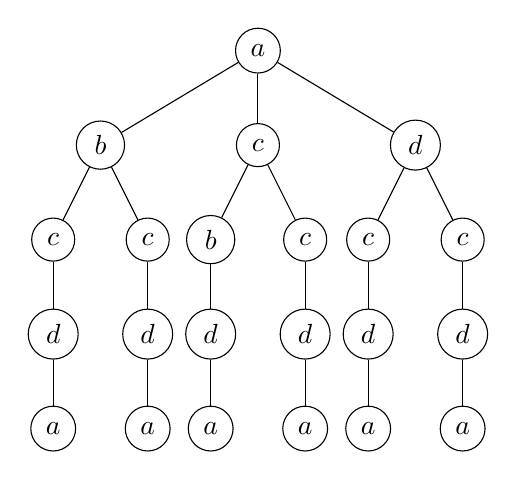
\begin{tikzpicture}[sibling distance=10em,
  every node/.style = {shape=circle, rounded corners,
    draw, align=center,
    top color=white, bottom color=white!5}, scale=0.8]
    \tikzstyle{level 1}=[sibling distance=25mm] 
    \tikzstyle{level 2}=[sibling distance=15mm] 
    \tikzstyle{level 3}=[sibling distance=10mm] 
    
  \node {$a$}
    child { node {$b$} 
        child {node {$c$}
        child {node {$d$}
        child {node {$a$}}}}
        child {node {$c$}
        child {node {$d$}
        child {node {$a$}}}}}
    child { node {$c$} 
        child {node {$b$}
        child {node {$d$}
        child {node {$a$}}}}
        child {node {$c$}
        child {node {$d$}
        child {node {$a$}}}}}
    child { node {$d$} 
        child {node {$c$}
        child {node {$d$}
        child {node {$a$}}}}
        child {node {$c$}
        child {node {$d$}
        child {node {$a$}}}}};
\end{tikzpicture}
\end{center}
The idea behind the exhaustive, brute-force approach is to traverse each path in the tree and then decide, this creates a very large problem to solve. The idea behind the dynamic approach is to start from the level 4 of the tree, which means we are now at the last vertex in the path and the next vertex from that completes the cycle and takes us back to the source node. This forms the smallest sub problem in the dynamic program. The next step would be go a level higher in the tree, which means we will now check the path length if we are reaching the source node from vertex $v$ and, we are reaching reaching vertex, $v$, from vertex, $u$ s.t. $u,v \in V$ where $V$ is the set of all vertices. We will keep doing this, and at each level we will decide the minimum path length of between n paths that are emerging from one vertex, this is done until the source node of the tree is reached, resulting in the minimum path. The dynamic algorithm can be generalised as a cost function, $g$, as follows:
$$g(i, S) = min_{k\in S} \bigg\{c_{ik} + g(k, S-\{k\})\bigg\}$$
s.t. $i$ is the source vertex, $S$ is the set of all vertices, $c_{ik}$ is the cost of some going from vertex $i$ to $k$. 
	
\subsubsection{Held-Karp Algorithm}
		
		
		
	\subsection{ Approximate Solutions}
		\subsubsection {Nearest Neighbour Algorithm}
    \subsubsection {Pairwise Exchange Method}

     First proposed in 1958 by G A Croes, It is a local search algorithm that iteratively optimizes an arbitrary path. The algorithm works by iterating over all possible combination of two edges that do not share common vertices and replacing them with another edge in a manner such that the total weight of the new edges is less than the total weigt of the deleted edges.
    Take the following two edges $u$ and $v$ and let their weights be $w_{1}$ and $w_{2}$ (The complete graph is not shown):
  \begin{center}
    \begin{tikzpicture}[auto, node distance=3cm, every loop/.style={},thick,main node/.style={circle,draw,font=\sffamily\Large\bfseries}]

      \node[main node] (1) {$u_{1}$};
      \node[main node] (2) [below of=1] {$v_{1}$};
      \node[main node] (3) [below of=2] {$v_{2}$};
      \node[main node] (4) [below right of=1] {$u_{2}$};
      
    
      \path[every node/.style={font=\sffamily\small}]
        (1) edge node [left] {edge $u$,weight $w_1$} (4)
    
        (3) edge node [right] {edge $v$,weight $w_2$} (2);

    First proposed in 1958 by G A Croes, It is a local search algorithm that iteratively optimizes an arbitrary path. The algorithm works by iterating over all possible combination of two edges that do not share a common vertices and replacing them in a particular manner.
    Take the following two edges (1,4) and (2,3):
  \begin{center}
    \begin{tikzpicture}[auto, node distance=3cm, every loop/.style={},thick,main node/.style={circle,draw,font=\sffamily\Large\bfseries}]

      \node[main node] (1) {1};
      \node[main node] (2) [below of=1] {2};
      \node[main node] (3) [below of=2] {3};
      \node[main node] (4) [below right of=1] {4};
      
    
      \path[every node/.style={font=\sffamily\small}]
        (1) edge node [left] {$w_{1}$} (4)
    
        (3) edge node [right] {$w_{2}$} (2);

        
    \end{tikzpicture}
  \end{center}

    Pairwise exchange will select these two edges and replace them with edges such that the new edges are $uv_{1}$ and $uv_{2}$:
    \begin{center}
    \begin{tikzpicture}[auto, node distance=3cm, every loop/.style={},thick,main node/.style={circle,draw,font=\sffamily\Large\bfseries}]

      \node[main node] (1) {$u_{1}$};
      \node[main node] (2) [below of=1] {$v_{1}$};
      \node[main node] (3) [below of=2] {$v_{2}$};
      \node[main node] (4) [below right of=1] {$u_{2}$};
      
    
      \path[every node/.style={font=\sffamily\small}]
        (1) edge node [left] {edge $uv_{1}$,weight $w_3$} (2)
    
        (3) edge node [right] {edge $uv_{2}$,weight $w_4$} (4);

    Pairwise exchange will select these two edges and replace them with edges such that the new edges are (1,2) and (3,2):
    \begin{center}
    \begin{tikzpicture}[auto, node distance=3cm, every loop/.style={},thick,main node/.style={circle,draw,font=\sffamily\Large\bfseries}]

      \node[main node] (1) {1};
      \node[main node] (2) [below of=1] {2};
      \node[main node] (3) [below of=2] {3};
      \node[main node] (4) [below right of=1] {4};
      
    
      \path[every node/.style={font=\sffamily\small}]
        (1) edge node [left] {$w_{3}$} (2)
    
        (3) edge node [right] {$w_{4}$} (4);

    
    
        
    \end{tikzpicture}
    \end{center}
    

    The following condition is checked, everytime an edge exchange is done:
    
    \[w_{3}+w_{4} - (w_{1} +w_{2})<0\]
    
    The sum of weights of the two new edges and the deleted edges is subtracted to see if there has been a decrease or not. If replacing the edges brings about a decrease in the total weight, then the replaced edges are preserved. Otherwise, the old edges are kept and some other combination of edges are tested for replacement. The Algorithm below states the exact steps that we need to make:\\
    
    \begin{algorithm*}
        \KwIn{A weighted complete graph $G$}
        \KwOut{An optimized Hamiltonian path $best_p$}
        Initialize an arbitrary path p \\
        $best_p$=p \\
        While $best_p$ improves: \\
        for $i$ in range(1,length($p.vertices$)-2): \\
        \quad for $j$ in range(i+1,length($p.vertices$)):\\
        \qquad if best($u_{1}$,$v_{1}$)+best($u_{2}$,$v_{2}$)$-$(best($u_{1}$,$u_{2}$)+best($v_{1}$,$v_{2}$)) $<$ 0:\\
        swap edges from $u$,$v$ to $uv_{1}$ and $uv_{2}$\\
    \Return{\upshape the hamiltonian path $best_p$}
    \caption{\textsc{Pairwise Exchange Method}}
    \end{algorithm*}        
    
    Each time the algorithm runs, it checks for each possible edge exchange in a given Hamiltonian path and seeks to decrease the total weight of the path. Hence, each time the Algorithm runs, a new path is produced whose total weight may be further minimized. Although, a $termination condition$ may be added to let the outer while loop run for a specified number of sequences before giving out the result in order to avoid having to search across all possible n! paths.

    The sum of weights of the two new edges and the deleted edges is compared to see if there has been a decrease or not. If replacing the edges brings about a decrease in the total weight, then the replaced edges are preserved. Otherwise, the old edges are kept and some other combination of edges are tested for replacement.

    \newpage
    \subsubsection {Christofides–Serdyukov Algorithm}
    The Christofides–Serdyukov algorithm is another approximation algorithm, that gives a solution that is 
    relatively close to the optimal TSP tour. First, we will take a look at a simpler approximation 
    algorithm that results in an approximation ratio of 2.

    \begin{algorithm*}
      \KwIn{A weighted complete graph $G$ and a root vertex $v$}
      \KwOut{A hamiltonian cycle $H$.}
      compute a minimum spanning tree $T$ for $G$ using \textsc{MST-PRIM}($G, v$) \\
      let $H$ be the list of vertices, ordered according to when they are first visited in a
      preorder tree walk of $T$ \\
      \Return{\upshape the hamiltonian cycle $H$}
  \caption{\textsc{approx-tsp-tour}}
  \end{algorithm*}
    
  This algorithm relies on the assumption that the weights of the edges of the graph conform to the triangle inequality and that the graph is complete.
  Let $c(u,v)$ be the weight of 
  an edge. Then, \[c(u,w) \leq c(u,v) + c(v, w) \]
  In simpler words, removing an intermediate stop would never increase the cost. If the edges do not conform to the triangle inequality, then a polynomial-time approximation
  with a constant approximation ratio does not exist, unless $\P = \NP$. The proof of this
  is outside the scope of this paper. This version of the TSP is also called a metric TSP since 
  the edge weights form a metric space.   
  \paragraph{} Let's look at a short proof that \textsc{approx-tsp-tour} is a poly-time 2- approximation algorithm. 
  \begin{proof}
    Let $H^*$ denote the optimal TSP tour for a set of vertices. We can obtain a spanning tree $T$ by eliminating an edge from 
    $H^*$. This provides a lower bound for cost of $H*$. 
    \[c(T) \leq c(H^*)\] A full walk $W$ of $T$ would visit every edge of $T$ twice, which means   
    \[c(W) = 2\cdot c(T) \implies c(W) \leq 2\cdot c(H^*)\]
  Since, the triangle inequality is being obeyed, we can remove repeated visits in $W$ with a guarantee that 
  the cost will not increase.
  Let $H$ be the cycle corresponding to a pre-order walk in $T$. This hamiltonian cycle is the cycle that is computed by 
  \textsc{approx-tsp-tour}. Since $H$ is obtained by deleting vertices from $W$,
  \[c(H) \leq c(W)\]
  This implies that, \[c(H) \leq 2\cdot c(H^*)\] which completes the proof. 
  \end{proof}

  {\large{\textbf{An Improved Algorithm:}}}  \paragraph{}
  
  This algorithm can be improved by adding a few more graph operations that can further optimize our solution.
  The improved algorithm by Christofides relies on the same assumptions (triangle inequality and complete graph). 
  However, it utilizes other graph properties to improve the approximation ratio. These facts/properties are:
  \begin{enumerate}
    \item[Fact 1:] The number of vertices with odd degree in a graph is always even, according to the handshaking lemma. 
    \item[Fact 2:] A graph that has all vertices with even degree will have an Eulerian tour. 
    \item[Fact 3:] Given a complete weighted graph with an even number of vertices, a minimal weight perfect matching can be found in polynomial 
     time. Specifically, it can be computed in $O(|E||V|^2)$  using the Blossom algorithm by Jack Edmonds.
  \end{enumerate} 
  \begin{algorithm*}
    \KwIn{A weighted, complete graph $G$, and a root vertex $v$.}
    \KwOut{A circuit $\Gamma$}
    compute a minimum spanning tree $T$ for $G$ using \textsc{mst-prim}($G, v$) \\
    let $O$ be the set of vertices with odd degree in $T$ \\
    find an induced subgraph $G'$ given by vertices in $O$ \\
    find a minimum-weight perfect matching $M$ in $G'$ \\
    combine the edges of $M$ and $T$ to form an Eulerian multigraph $M^*$ \\
    find an Eulerian circuit $\Gamma$ in $M^*$ \\
    make $\Gamma$ a Hamiltonian cycle by skipping repeated vertices \\
    \Return{\upshape the Hamiltonian cycle $H$}
    \caption{\textsc{Christofides-Seryukov}}
\end{algorithm*}

  
\section{Theoretical Runtime Analysis and Comparison}
\subsection{Pairwise Exchange Method}
Each time a while loop runs, it takes a total $O(n^2)$ times. The while loop in itself will only stop when the total weight of the hamiltonian patn converges to an optimal value. In theory, the while loop does not converge at all. Every time we get a path, we can iterate over all of the possible edge exchanges to optimize the path, so this algorithm is an exhaustive search over all of the possible optimal solutions. Hence, the time complexity is O(n!).
=======
  Initially, a minimum spanning tree $T$ is constructed. Then from $T$, we add vertices with odd degree to the set $O$. 
  Then we create a subgraph: $G' = G[O]$, i.e. a subgraph induced by the vertices in $O$. Due to Fact 1, this subgraph has 
  even number of vertices. We then find a minimum weight perfect matching $M$ on $G'$, add this matching to the MST $T$, creating 
  an Eulerian multigraph $M^*$. This multigraph will have all vertices having an even degree. This makes it possible for us 
  to find an Eulerian circuit $\Gamma$ in $M^*$. We then reduce $\Gamma$ to a Hamiltonian circuit using the triangle inequality 
  property to remove repeated vertices. The resulting circuit is our approximate solution to the problem. 
  \paragraph{}
  This algorithm is a $\frac{3}{2}$-approximation algorithm. Let us look at the proof of this. 
  \begin{proof}
    Let $H^*$ be the optimal TSP tour and $c(H^*)$ be its weight. 
    Since $T$ is an MST in $G$, \[c(T) \leq c(H^*)\] 
    Let $R$ be the solution to the TSP problem on subgraph $G'$. This means that $c(R) \leq c(H^*)$. We can partition the minimum weight perfect matching 
    on subgraph $G'$. The cost of these partitions is going to sum to $c(R)$; therefore, the smaller of these two partitions is 
    going to be at most $c(R)/2$. Since $M$ is a minimum weight perfect matching on $G'$, will be at most smaller than the partitions of $R$. 
    Therefore, \[c(M) \leq \frac{c(R)}{2}\]
    And so, \[c(T) + c(M) \leq c(H^*) + \frac{c(R)}{2} \leq \frac{3}{2} \cdot c(H^*)\]
    Because of the triangle inequality, short cuts will lead to a better cost. Therefore, 
    \[c(H) \leq c(T) + c(M) \] where $H$ is the approximate tour returned by the Christofides-Seryukov algorithm. This leads to
    \[c(H) \leq \frac{3}{2} \cdot c(H^*)\]
    which concludes our proof.
  \end{proof}

  \textbf{Analysis:} \paragraph{}
  \textsc{approx-tsp-tour} is an $O(n)$ algorithm since all operations in this algorithm are linear and if Prim's algorithm is 
  implemented using adjacency lists and binary heaps. Otherwise, Prim's algorithm would be $O(n^2)$ in the 
  case of adjacency matrix and would dominate the runtime of \textsc{approx-tsp-tour} making it $O(n^2)$.
  \paragraph{} The time complexity of the Christofides–Serdyukov algorithm depends on the most expensive operation in the 
  algorithm - finding a minimum weight perfect matching (line 4). This operation is implemented using the Blossom algorithm, which is $O(n^3)$. All the other 
  processes are linear, which means that this algorithm would be $O(n^3)$, where $n$ is the number of vertices. 

  \section{Theoretical Runtime Analysis and Comparison}

    \subsection{Pairwise Exchange Method}
Each time a while loop runs, it takes a total $O(n^2)$ times. The while loop in itself will only stop when the total weight of the hamiltonian path converges to an optimal value. In principal, the algorithm is doing an exhaustive search through all the possible hamiltonian paths of a graph. Every time we get a path, we can iterate over all of the possible edge exchanges to optimize the path. As stated in section 2.1, there are n! hamiltonian paths to iterate over in total. Hence, the time complexity is $O(n!)$.
=======

\section{Empirical Runtime Analysis and Comparison}
\section{Conclusion}
\newpage
\section{References}
\begin{enumerate}
	\item \url{https://www.researchgate.net/publication/289195926_On_the_Nearest_Neighbor_Algorithms_for_the_Traveling_Salesman_Problem}
	\item \url{https://en.wikipedia.org/wiki/Travelling_salesman_problem#:~:text=The%20travelling%20salesman%20problem%20}
	\item Thomas H. Cormen, Charles E. Leiserson, Ronald L. Rivest, and Clifford Stein. 2009. Introduction to Algorithms, Third Edition (3rd. ed.)
	\item David L. Applegate, Robert E. Bixby, Vasek Chvatal, and William J. Cook. 2007. The Traveling Salesman Problem: A Computational Study. Princeton University Press, USA.
	\item Michael T. Goodrich, Roberto Tamassia. 2014. Algorithm Design and Applications. Wiley, USA. 
	\item Christofides. 1976. Worst-case analysis of a new heuristic for the travelling salesman problem, Report 388, Graduate School of Industrial Administration, CMU.
\end{enumerate}




\end{document}
